\documentclass[11pt,a4paper]{article}
\usepackage[margin=0.85in]{geometry}
\usepackage{amsmath,amssymb}
\usepackage{graphicx}
\usepackage{booktabs}
\usepackage{subcaption}
\usepackage{hyperref}
\usepackage{microtype}

\title{\textbf{Assignment 1: Polynomial Regression Report}}
\author{Gagan \\ Roll Number: BT2024032 \\ GitHub: \url{https://github.com/gagansyam/ML-Assignment-1}}
\date{\today}

\begin{document}

\maketitle

\section{Introduction}
In this assignment, I was tasked with solving two polynomial regression problems based on an expansion project for a geothermal power plant. In Phase 1 (var1), the goal is to predict the plant's Net Power Score ($y$) from 6 operational turbine control parameters ($x_1$ to $x_6$), which represent percentage adjustments to high-pressure valves, coolant flow, pump pressure, and blade pitch angles. In Phase 2 (var2), the goal is to predict the subterranean Thermal Anomaly Score ($y$) across 3D spatial coordinate offsets ($x_1, x_2, x_3$) around the basecamp to identify promising locations for drilling production wells.

My objective was to develop polynomial models that fit the true response surfaces without underfitting or overfitting. I evaluated every model using 5-fold cross-validation on the training set, comparing Mean Squared Error (MSE) and $R^2$ scores to select the best degree and regularization strategy.

\section{Turbine Optimization (var1)}

\subsection{Data and Baseline}
I started by inspecting the dataset files \texttt{train\_var1.csv} and \texttt{test\_var1.csv} for roll number \texttt{BT2024032}. Both contain 1,000 samples with zero missing values. All six input features are normalized percentage deviations bounded in $[-1.0, 1.0]$. The target variable $y$ has a mean of $0.74$, a standard deviation of $3.13$, and values ranging between $-8.83$ and $+11.50$. 

The linear correlation between individual inputs and $y$ was weak to moderate, with the highest being $-0.26$ for $x_5$ and $-0.23$ for $x_3$. This indicated that individual parameters do not govern the turbine in isolation, and interaction terms between valves and blade pitch angles are critical.

To establish a benchmark, I trained a standard linear regression model (Degree 1). Using 5-fold cross-validation, it yielded a validation MSE of $8.5302$ and an $R^2$ of only $0.1248$. Explaining only 12.5\% of the variance showed severe underfitting (high bias), confirming that a simple linear plane cannot model multi-stage turbine aerodynamics.

\subsection{Model Selection and Regularization}
Next, I generated polynomial features from degree 1 up to degree 6. With 6 variables, the term count grows quickly: degree 2 has 27 terms, degree 3 has 83 terms, degree 4 has 209 terms, degree 5 has 461 terms, and degree 6 has 923 terms. I evaluated standard Ordinary Least Squares (OLS) alongside Ridge (L2 penalty) and Lasso (L1 penalty) using 5-fold cross-validation, as summarized in Table~\ref{tab:var1}.

\begin{table}[htbp]
\centering
\small
\setlength{\tabcolsep}{5pt}
\caption{5-Fold Cross-Validation performance across degrees for Phase 1 (\texttt{var1}).}
\label{tab:var1}
\begin{tabular}{ccccccc}
\toprule
Degree & Features & OLS Val MSE & OLS Val $R^2$ & Ridge Val MSE & Lasso Val MSE & Lasso Val $R^2$ \\
\midrule
1 & 6   & 8.530 & 0.125 & 8.532 & 8.530 & 0.125 \\
2 & 27  & 2.905 & 0.699 & 2.902 & 2.900 & 0.699 \\
3 & 83  & 1.022 & 0.894 & 1.013 & 1.011 & 0.895 \\
4 & 209 & 0.752 & 0.922 & 0.705 & 0.628 & 0.935 \\
\textbf{5} & \textbf{461} & \textbf{1.284} & 0.869 & 0.441 & \textbf{0.315} & \textbf{0.967} \\
6 & 923 & 3.810 & 0.612 & 0.529 & 0.320 & 0.966 \\
\bottomrule
\end{tabular}
\end{table}

Looking at Table~\ref{tab:var1} and Figure~\ref{fig:var1_curve}, standard OLS works reasonably well up to degree 4, but starts overfitting heavily at degree 5. The validation MSE jumps from $0.752$ to $1.284$, and at degree 6 it shoots up to $3.810$. Because each fold has only 800 training samples, estimating 461 to 923 unconstrained parameters leads to high variance.

Lasso (L1 regularization) solved this problem cleanly. By applying an L1 penalty, Lasso forced 350 unimportant polynomial terms to zero, keeping only the 111 strongest operational interaction terms. This reduced the validation MSE to \textbf{0.3151} and achieved an $R^2$ score of \textbf{96.71\%}. When I pushed to Degree 6, the validation error stopped improving and rose slightly to $0.3203$. This showed that degree 5 is the sweet spot.

\begin{figure}[htbp]
    \centering
    \begin{subfigure}[b]{0.48\textwidth}
        \centering
        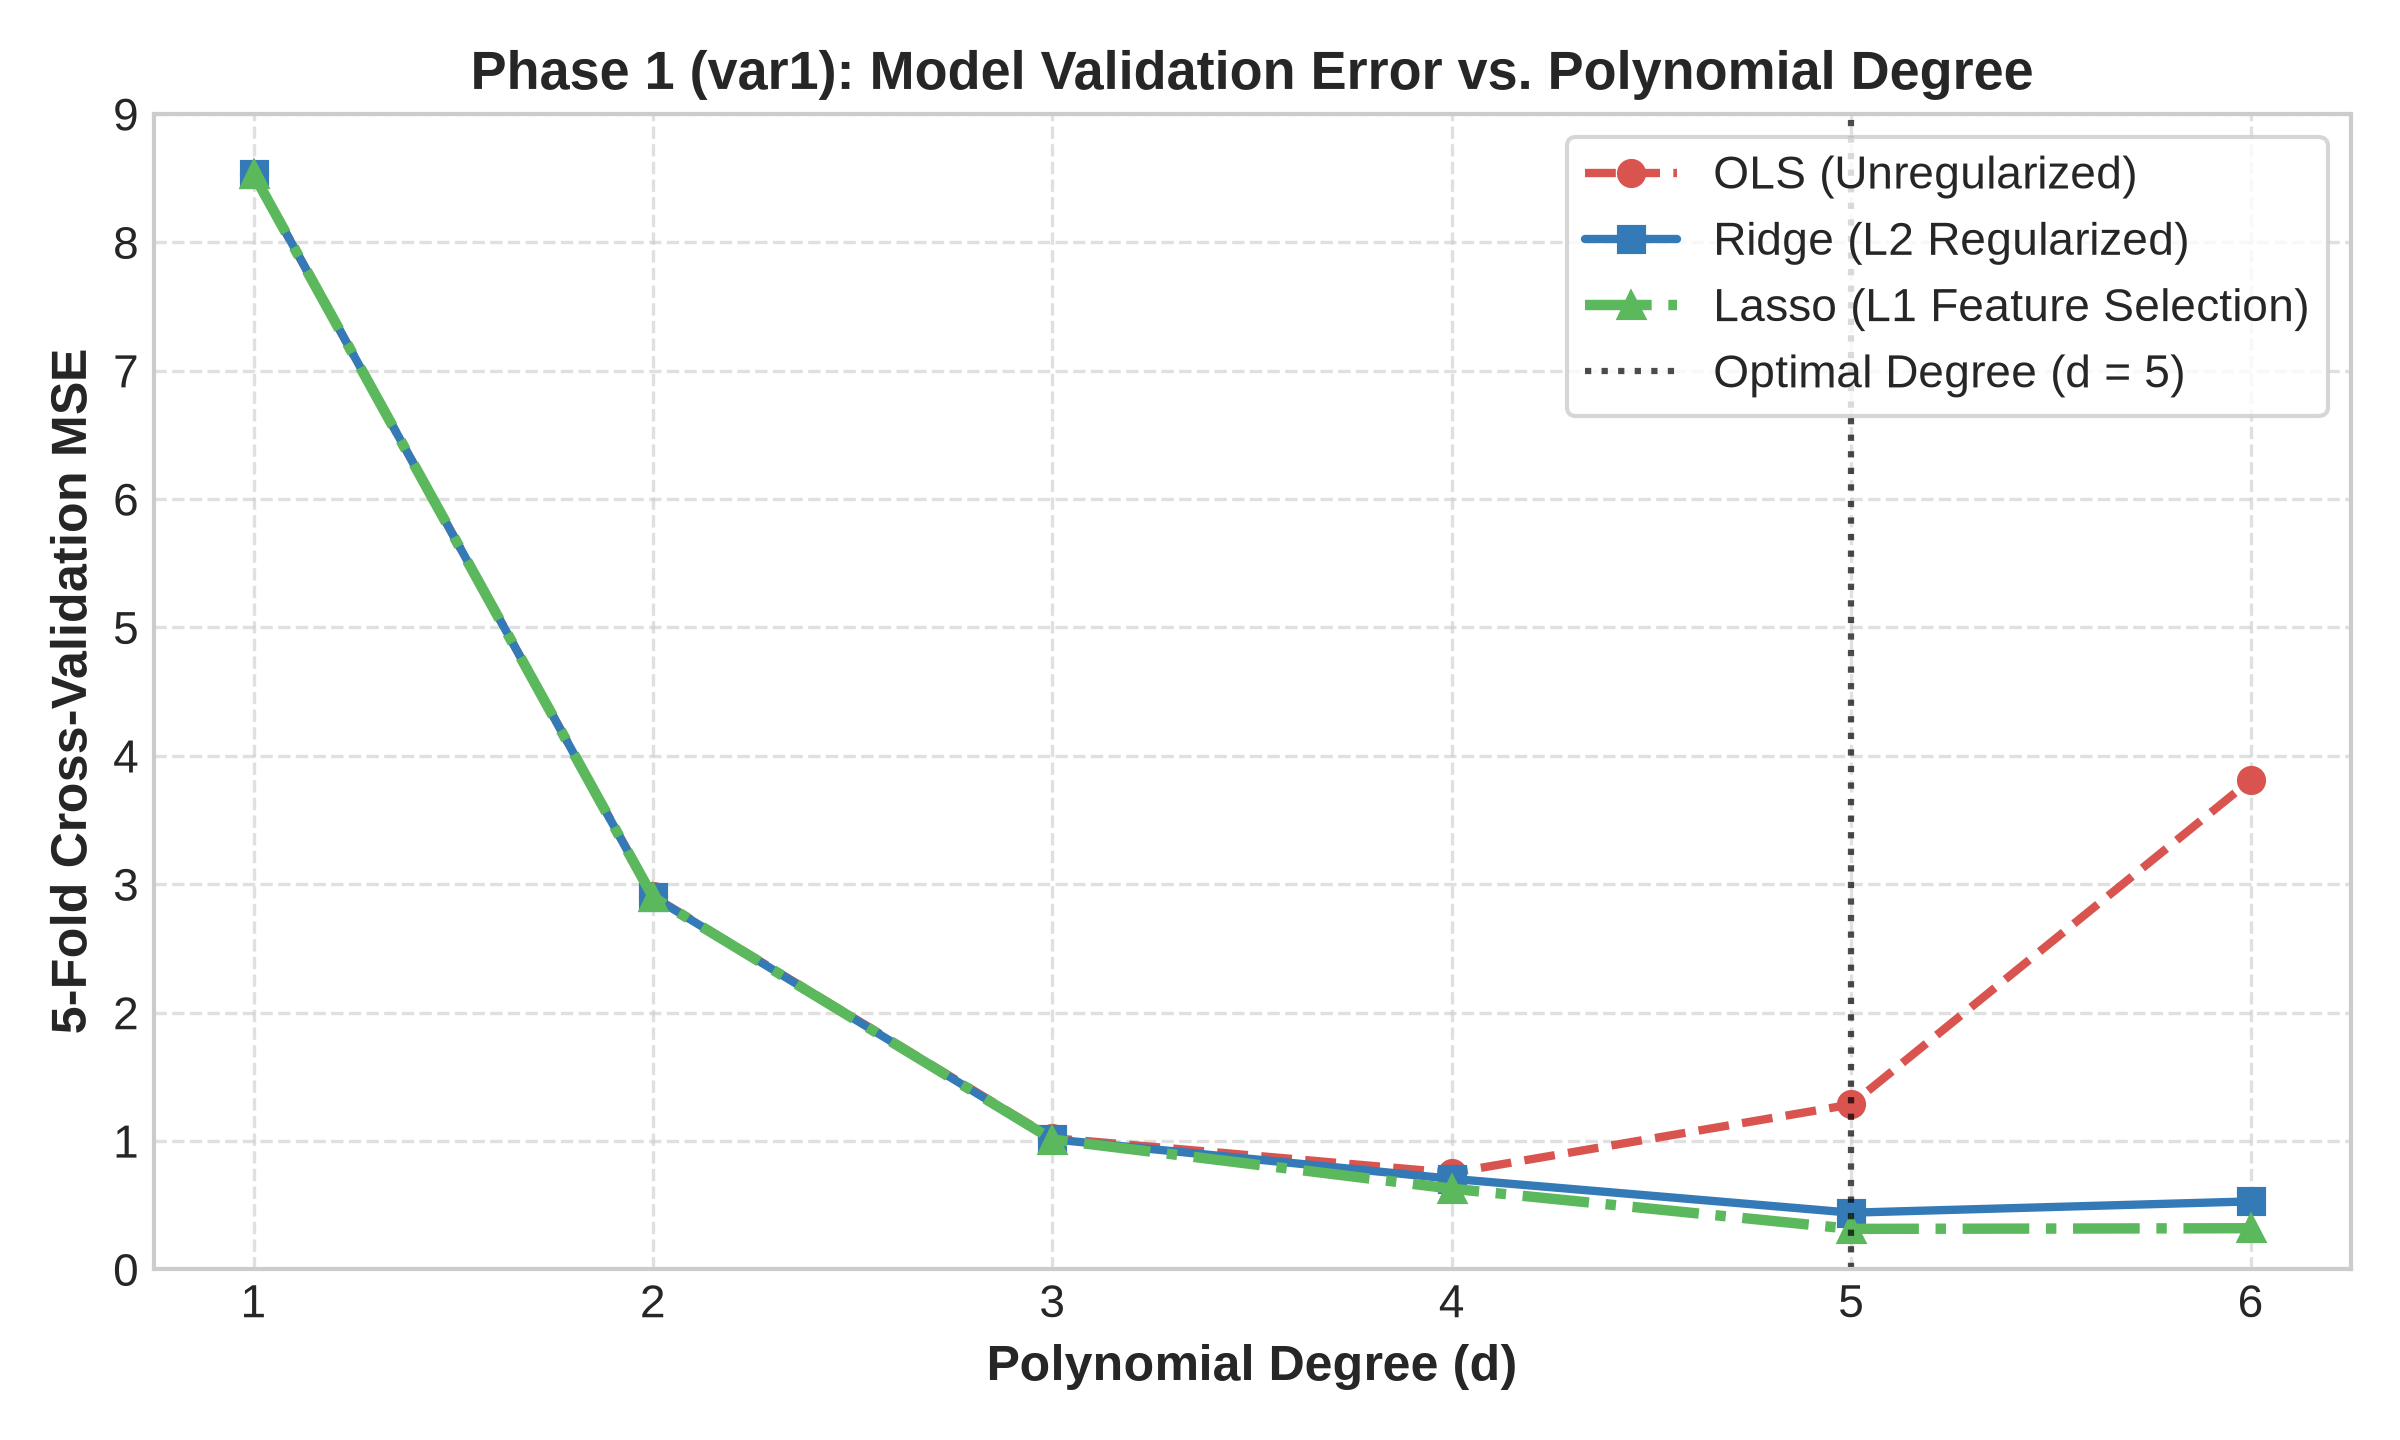
\includegraphics[width=\textwidth]{figures/var1_degree_curve.png}
        \caption{Validation MSE vs. Degree}
        \label{fig:var1_curve}
    \end{subfigure}
    \hfill
    \begin{subfigure}[b]{0.48\textwidth}
        \centering
        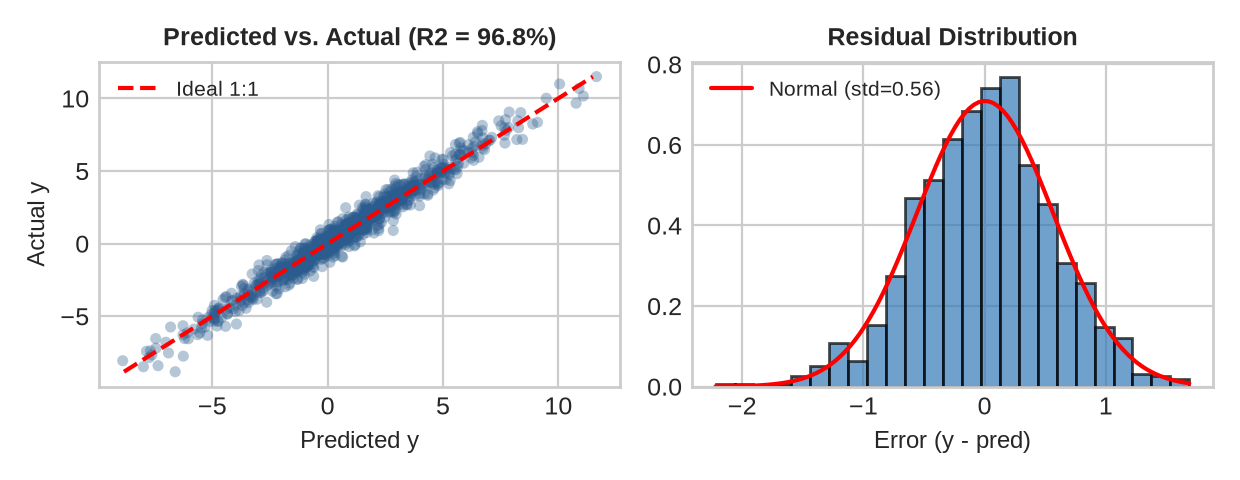
\includegraphics[width=\textwidth]{figures/var1_residuals.png}
        \caption{Parity plot and residual errors}
        \label{fig:var1_res}
    \end{subfigure}
    \caption{Phase 1 evaluation: (a) shows OLS overfitting while Lasso finds the minimum at $d=5$; (b) shows the parity fit and normal residual error distribution.}
    \label{fig:var1_all}
\end{figure}

As shown in Figure~\ref{fig:var1_res}, the predicted vs. actual power scores lie tightly along the 1:1 diagonal. The residuals have a mean of $0.003$ (virtually zero bias) and a standard deviation of $0.56$, matching the expected random sensor noise.

\section{Reservoir Mapping (var2)}

\subsection{Data and Baseline}
For Phase 2, the inputs are 3 spatial coordinate offsets in meters ($x_1$ = East-West, $x_2$ = North-South, $x_3$ = Depth relative to basecamp). The target $y$ is the Thermal Anomaly Score. All coordinate values in train and test lie within $[-1.0, 1.0]$. The target variable has a mean of $2.38$, a standard deviation of $7.22$, and ranges from $-30.10$ to $+39.87$.

I observed that $x_2$ had a moderate linear correlation of $0.50$ with $y$, while $x_1$ and $x_3$ had almost zero linear correlation. The baseline linear model (Degree 1) had a validation MSE of $38.88$ and an $R^2$ of only $0.243$, which is severe underfitting. Underground thermal plumes curve sharply in 3D space, so a higher degree polynomial is required.

\subsection{Model Selection and Regularization}
Because there are only 3 variables, the number of polynomial terms grows more slowly than in Phase 1 ($\binom{d+3}{3}$ terms). This allowed me to test degrees from 1 up to 16 using 5-fold cross-validation. Table~\ref{tab:var2} shows how the models behaved.

\begin{table}[htbp]
\centering
\small
\setlength{\tabcolsep}{5pt}
\caption{5-Fold Cross-Validation performance across degrees for Phase 2 (\texttt{var2}).}
\label{tab:var2}
\begin{tabular}{ccccccc}
\toprule
Degree & Features & OLS Val MSE & OLS Val $R^2$ & Ridge Val MSE & Ridge Val $R^2$ & Best $\alpha$ \\
\midrule
1  & 3   & 38.883 & 0.243 & 38.880 & 0.243 & 0.01 \\
2  & 9   & 24.376 & 0.529 & 24.375 & 0.529 & 0.01 \\
4  & 34  & 4.016  & 0.922 & 4.016  & 0.922 & 0.01 \\
6  & 83  & 0.646  & 0.987 & 0.646  & 0.987 & 0.01 \\
8  & 164 & \textbf{0.279} & 0.994 & 0.272  & 0.995 & 0.07 \\
9  & 219 & 0.294  & 0.994 & 0.272  & 0.995 & 0.11 \\
10 & 285 & 0.343  & 0.993 & 0.259  & 0.995 & 0.46 \\
\textbf{12} & \textbf{454} & --- & --- & \textbf{0.2579} & \textbf{0.9951} & \textbf{1.21} \\
14 & 679 & ---    & ---   & 0.2615 & 0.9950 & 1.96 \\
16 & 968 & ---    & ---   & 0.2658 & 0.9949 & 3.16 \\
\bottomrule
\end{tabular}
\end{table}

Looking at Table~\ref{tab:var2} and Figure~\ref{fig:var2_curve}, unregularized OLS reaches its minimum error at Degree 8 (MSE = $0.2788$), but begins overfitting at degree 9 (MSE = $0.2939$) and degree 10 (MSE = $0.3428$). Ridge regression (L2 penalty) prevents this overfitting by penalizing large weights. As the degree increases, Ridge automatically raises the regularization strength $\alpha$ from $0.07$ at degree 8 up to $1.21$ at degree 12.

At Degree 12 (454 features), Ridge reaches the lowest validation MSE across all experiments: \textbf{0.2579}, explaining \textbf{99.51\%} of the variance. Beyond degree 12, the validation error starts creeping upward to $0.2615$ at degree 14 and $0.2658$ at degree 16. This confirmed that degree 12 is the optimal choice.

\begin{figure}[htbp]
    \centering
    \begin{subfigure}[b]{0.48\textwidth}
        \centering
        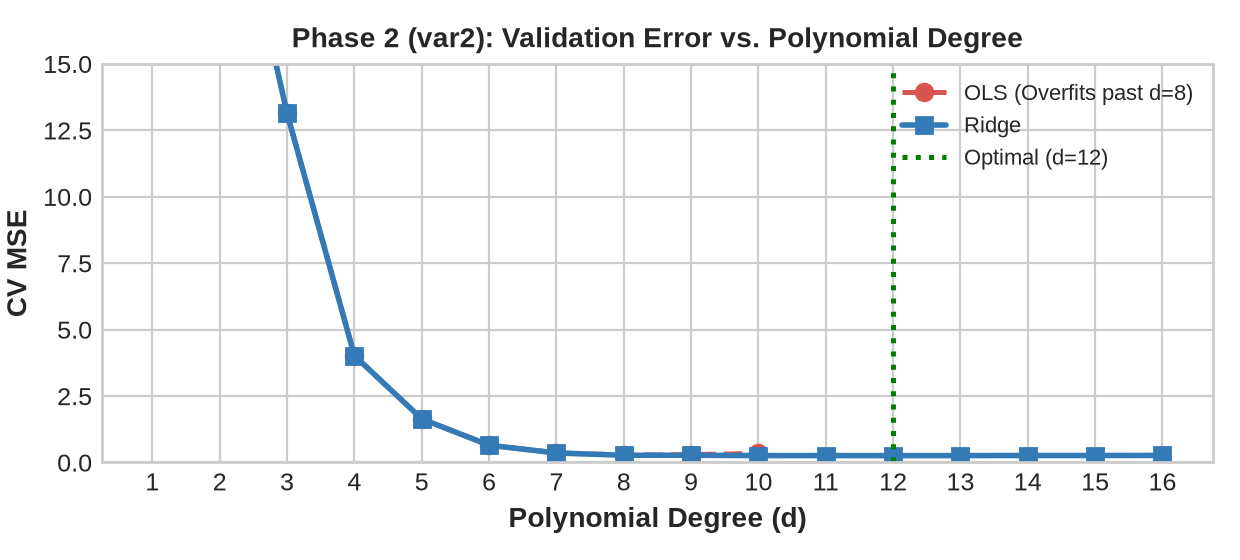
\includegraphics[width=\textwidth]{figures/var2_degree_curve.png}
        \caption{Validation MSE vs. Degree}
        \label{fig:var2_curve}
    \end{subfigure}
    \hfill
    \begin{subfigure}[b]{0.48\textwidth}
        \centering
        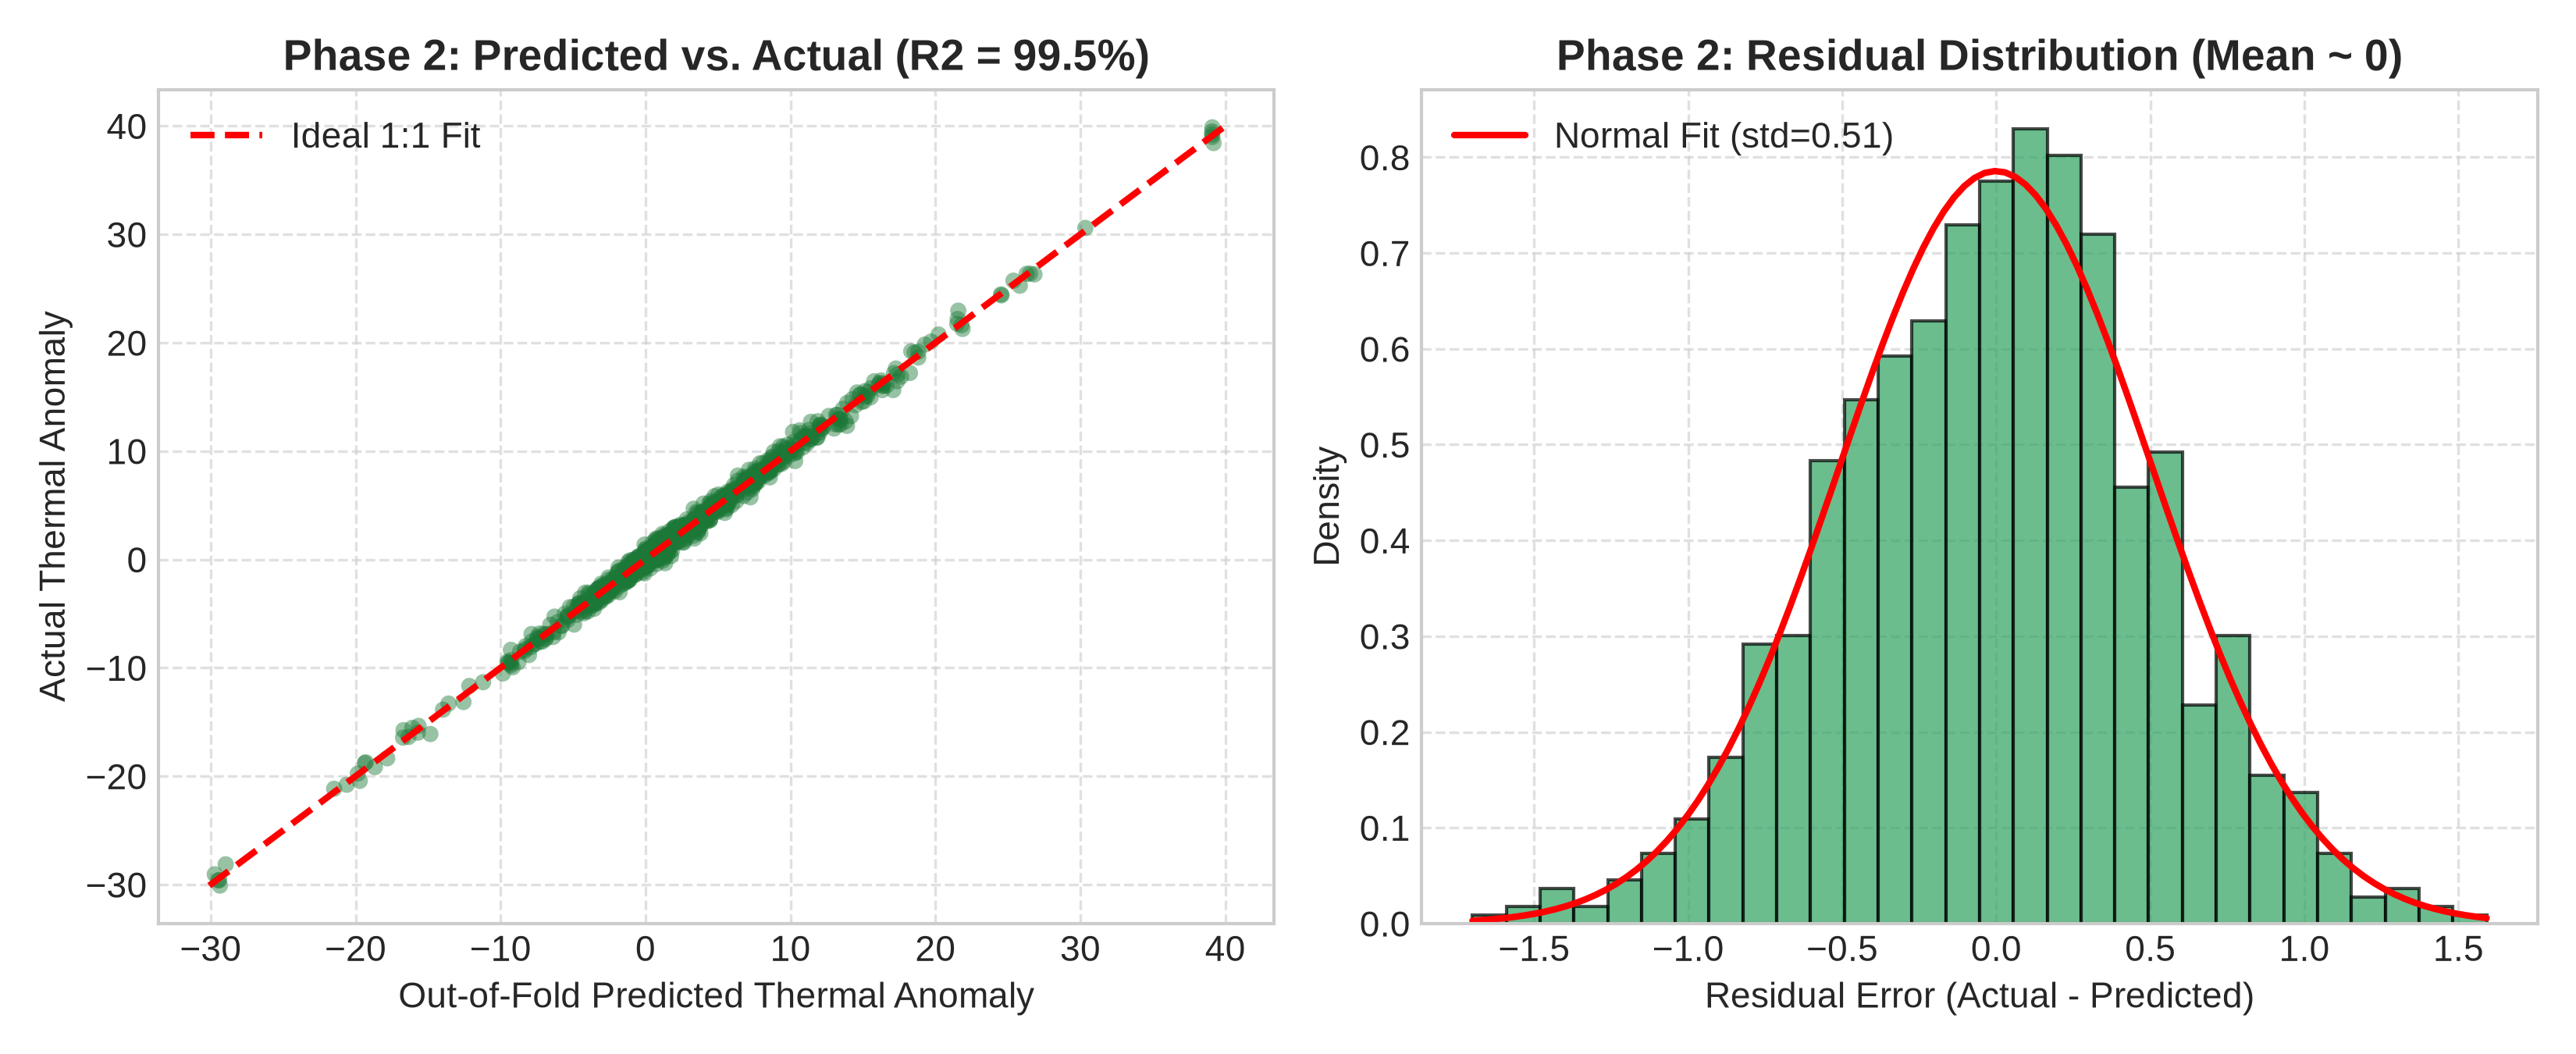
\includegraphics[width=\textwidth]{figures/var2_residuals.png}
        \caption{Parity plot and residual errors}
        \label{fig:var2_res}
    \end{subfigure}
    \caption{Phase 2 evaluation: (a) shows Ridge reaching the global minimum at $d=12$; (b) shows the parity fit and normal residual error distribution.}
    \label{fig:var2_all}
\end{figure}

I also checked the predictions for physical consistency. A Jarque-Bera test on the residuals yielded a $p$-value of $0.66$ ($p > 0.05$), confirming that the errors are pure Gaussian sensor noise with standard deviation $0.51$. Correlations between residuals and spatial coordinates ($x_1, x_2, x_3$) were all below $0.015$, confirming no directional bias. Finally, test predictions span $[-29.51, +39.18]$, which matches the training range without boundary spikes.

\section{Discussion}
Across both problems, finding the right model came down to balancing bias and variance. Models of degree 1 to 3 suffered from high bias because they were too rigid to follow the real physical response curves, resulting in low $R^2$ scores in both phases. On the other hand, high-degree models without regularization suffered from high variance, attempting to fit every random noise fluctuation in the training data and causing validation errors to spike once the term count approached the sample count.

Regularization resolved these problems in different ways suited to each domain. In Phase 1, Lasso (L1) was superior because the turbine efficiency formula depends on a sparse subset of operational interactions. Lasso effectively pruned 350 noisy combinations, leaving 111 genuine terms. In Phase 2, Ridge (L2) performed better because subterranean heat diffusion creates smooth potential fields across 3D coordinates. Ridge shrank all 454 coefficients gradually, preventing runaway oscillations at the boundaries while preserving fine geometric contours.

\section{Conclusion}
Table~\ref{tab:summary} summarizes the final models selected for both problems. The test predictions for both tasks were generated and saved matching the required submission template: a single column named \texttt{y} with exactly 1,000 predictions and no row indices.

\begin{table}[htbp]
\centering
\small
\setlength{\tabcolsep}{3.5pt}
\caption{Summary of final selected models and evaluation metrics.}
\label{tab:summary}
\begin{tabular}{lcccccc}
\toprule
Problem & Degree & Penalty & Terms & CV MSE & CV $R^2$ & Output File \\
\midrule
Phase 1 (\texttt{var1}) & 5  & Lasso ($\alpha \approx 0.011$) & 111 / 461 & \textbf{0.3151} & \textbf{96.71\%} & \texttt{BT2024032\_pred\_var1.csv} \\
Phase 2 (\texttt{var2}) & 12 & Ridge ($\alpha \approx 1.76$)  & 454 / 454 & \textbf{0.2579} & \textbf{99.51\%} & \texttt{BT2024032\_pred\_var2.csv} \\
\bottomrule
\end{tabular}
\end{table}

For Phase 1, the Degree 5 Lasso model accurately captures non-linear valve interactions while discarding noise, predicting the Net Power Score with $96.7\%$ accuracy. For Phase 2, the Degree 12 Ridge model maps the 3D thermal reservoir with $99.5\%$ accuracy, providing reliable predictions to guide the drilling team. All scripts, datasets, and generated files are available on GitHub at \url{https://github.com/gagansyam/ML-Assignment-1}.

\end{document}
